\documentclass[conference]{IEEEtran}
\IEEEoverridecommandlockouts
% The preceding line is only needed to identify funding in the first footnote. If that is unneeded, please comment it out.
%Template version as of 6/27/2024

\usepackage{cite}
\usepackage{amsmath,amssymb,amsfonts}

\usepackage{graphicx}
\usepackage{textcomp}
\usepackage{xcolor}
\usepackage{amsmath}
\usepackage{url}
\DeclareMathOperator*{\argmax}{arg\,max}
\usepackage{comment}

\usepackage{algorithm}
\usepackage{algpseudocode}
% A linha abaixo ajuda a posicionar o algoritmo onde ele é definido.
% Pode ser necessário \usepackage{float}
% \restylefloat{algorithm}

\usepackage{multirow}
\usepackage[normalem]{ulem}
\useunder{\uline}{\ul}{}

\def\BibTeX{{\rm B\kern-.05em{\sc i\kern-.025em b}\kern-.08em
    T\kern-.1667em\lower.7ex\hbox{E}\kern-.125emX}}
\begin{document}

\title{An Investigation into Multi-Task Learning for Point-of-Interest Category Classification and Next-POI Prediction  \\
}



\author{\IEEEauthorblockN{Vitor H. O. Silva, Ingred F. Almeida, Tarik S. Paiva, Germano B.\ Santos, Fabrício A.\ Silva, Felipe T. Sousa}
\IEEEauthorblockA{Laboratório de Inteligência em Sistemas Pervasivos e Distribuídos (NESPeD-LAB), UFV, Florestal, Brazil}
E-mail: \{vitor.h.oliveira, ingred.almeida,  tarik.paiva, germano.santos, fabricio.asilva, felipe.t.sousa\}@ufv.br
}

\maketitle

\begin{abstract}
Multi-Task Learning (MTL) has shown significant promise across various domains by improving generalization and robustness through shared representations. This work explores MTL within Location-Based Social Networks (LBSNs), focusing on two complementary tasks: POI Category Classification and Next-POI Prediction. We propose a joint MTL architecture that shares lower-level embeddings and sequence encoders while maintaining task-specific heads. Through experiments on the Gowalla LBSN dataset, we compare our MTL model against established single-task baselines. While our model demonstrated strong performance in POI category classification, outperforming the Human Mobility Representation Model (HMRM), the results for next-POI prediction were more competitive against MHA+PE. Crucially, our findings indicate that the multi-task learning approach did not consistently yield substantial improvements over the single-task baselines across both tasks, with many performance differences being minor and often within statistical standard deviations. Furthermore, contrary to expectations, the MTL model required significantly more computational resources and wall time to converge compared to the cumulative effort of individual single-task models. Our contributions include the introduction of a unified MTL framework for these POI-related tasks, the design of novel task-specific heads, and a detailed analysis of performance and convergence characteristics, highlighting observed limitations of MTL in this specific application. This research provides insights into the practical challenges of applying MTL, emphasizing the need for careful architectural design and optimization in achieving its theoretical benefits.
\end{abstract}

\begin{IEEEkeywords}
Multi-Task Learning, Point-of-Interest (POI), Location-Based Recommendation, Sequential Modeling
\end{IEEEkeywords}


%
% INTRODUCTION
%
% \section{Introduction}

% Multi-Task Learning (MTL) is a machine learning paradigm where multiple related tasks are learned jointly, sharing representations and inductive biases to improve generalization performance on each individual task \cite{caruana1997multitask}. By leveraging shared information across tasks, MTL has shown promise in mitigating overfitting, accelerating convergence, and yielding more robust feature extractors compared to single-task approaches.

% MTL has been successfully applied across a wide range of domains, including computer vision (e.g., joint object detection and segmentation) \cite{kokkinos2016ubernet}, natural language processing (e.g., joint part-of-speech tagging and named-entity recognition) \cite{wei2022finetuned}, healthcare (e.g., simultaneous diagnosis of multiple conditions) \cite{lipton2015learning}, and recommendation systems (e.g., modeling user preferences and item attributes together) \cite{zhang2020interactive}. 

% These successes motivate the exploration of MTL for Location-Based Social Network (LBSN), which encompass applications that utilize the geographical position of a mobile device to provide information and services. Within LBSN, Points-of-Interest (POIs) – specific physical locations that someone might find useful or interesting, such as restaurants, shops, or landmarks – are fundamental entities. Understanding and predicting user interactions with POIs are crucial, and related spatial prediction tasks in this domain may benefit significantly from shared geographic and temporal patterns.

% In this work, we study two complementary tasks in the context of POI recommendation and analysis:
% \begin{enumerate}
%   \item \textbf{POI Category Classification}: given the historical sequence of visited locations and their attributes, predict the semantic category (e.g., restaurant, museum) of each POI in a user’s trajectory.
%   \item \textbf{Next-POI Prediction}: given a prefix of a user’s trajectory, predict which POI category he/she will visit next, selecting from a finite set of possible categories.
% \end{enumerate}
% These tasks are closely related: accurate category features can inform next-location prediction, while trajectory modeling for next-POI prediction can improve category classification by capturing context and user intent. We, therefore, propose a joint MTL architecture that shares lower-level embeddings and sequence encoders, while maintaining task-specific heads.

% To evaluate our approach, we conducted experiments on the Gowalla LBSN, a real-world check-in dataset \cite{Cho2011, SNAP2014}. We compared our MTL model against established single-task baselines: Human Mobility Representation Model (HMRM) \cite{chen2020modeling} for POI category classification and MHA+PE \cite{zeng2019next} for next-POI prediction. While our proposed models demonstrated strong performance in POI category classification, outperforming HMRM across various metrics, the results for next-POI category prediction presented a more competitive landscape. Our MTL model achieved the best F1-scores in specific categories like Travel and Nightlife, but MHA+PE exhibited superior performance in others, such as Food and Shopping.

% Crucially, a direct comparison between our MTL and single-task models revealed that the multi-task learning approach did not yield the anticipated substantial and consistent improvements over the single-task baseline across both tasks. Many observed differences in F1-scores were minor and often fell within the reported standard deviations, suggesting that, statistically, the performance of the MTL and the Single-task models was largely comparable.



% The main contributions of this paper are as follows:
% \begin{itemize}
%   \item We introduce a MTL framework that simultaneously addresses POI category classification and next-POI prediction, sharing a similar embedding representation.\footnote{The complete source code, including hyperparameter configurations, is publicly available at \url{https://github.com/VitorHugoOli/PoiMtlNet} to ensure full reproducibility.}
%   \item We design novel task-specific heads that capture category co-occurrence patterns and sequential transition dynamics, respectively.
%   \item We conduct experiments using real-world check-in data from the state of Florida, evaluating the effectiveness of our MTL approach against single-task baselines across both tasks. Our analysis provides insights into performance trends and convergence behavior, emphasizing the practical implications and observed limitations of MTL in this context.
% \end{itemize}


% The rest of this paper is organized as follows. In Section~\ref{sec:related}, we review the theoretical foundations of MTL and prior work on POI modeling. Section~\ref{sec:methodology} describes our joint architecture, data preprocessing, and training protocol. Section~\ref{sec:experiments} presents experimental results. Finally, Section~\ref{sec:conclusion} summarizes our findings and discusses future research directions.

\section{Introduction}

Multi-Task Learning (MTL) is a machine learning paradigm where multiple related tasks are learned jointly, sharing representations and inductive biases to improve generalization performance \cite{caruana1997multitask}. By leveraging shared information, MTL can potentially mitigate overfitting and yield more robust feature extractors compared to single-task approaches. Its success in domains like computer vision \cite{kokkinos2016ubernet}, natural language processing \cite{wei2022finetuned} and recommendation systems \cite{zhang2020interactive} motivates its application to Location-Based Social Networks (LBSNs), where understanding user interactions with Points-of-Interest (POIs)  – specific physical locations that someone might find useful or interesting, such as restaurants, shops, or landmarks - is fundamental.

In this work, we investigate the application of MTL to two critical POI-related tasks:
\begin{enumerate}
    \item \textbf{POI Category Classification}: Classify the semantic category (e.g., shopping, travel) of a POI based on its features and context within a user's trajectory.
    \item \textbf{Next-POI Prediction}: Predicting the category of the next POI a user will visit, given the sequence of their prior visits.
\end{enumerate}

These tasks are ostensibly related, as both draw upon the same underlying user mobility data. Accurate POI category representations could inform next-location predictions, and conversely, sequential patterns could provide context for category classification. However, the tasks possess fundamentally different natures. POI Category Classification is primarily a \textbf{static classification task} that relies on the intrinsic, context-rich features of individual locations. In contrast, Next-POI Prediction is a \textbf{dynamic, sequential task} that depends on capturing temporal patterns and transitions.

This dichotomy raises a critical question: can a single, shared representation effectively serve two tasks with such distinct underlying characteristics? The assumption that MTL will be beneficial is not guaranteed. It is possible that forcing a shared encoder to learn features for both a static and a sequential task could result in \textbf{negative transfer}, where the joint training process actually hinders performance by learning a "compromise" representation that is not specialized enough for either task.

Therefore, the central hypothesis of this study is that a standard hard parameter-sharing MTL architecture will face significant limitations when applied to this specific task pairing, failing to achieve substantial and consistent improvements over well-tuned, specialized single-task models. Our work is thus framed as an empirical investigation into the boundary conditions of MTL's effectiveness, exploring whether the presumed task relatedness is sufficient to overcome their inherent structural differences.

To test this hypothesis, we conducted experiments on the Gowalla LBSN dataset \cite{Cho2011, SNAP2014}, comparing our MTL model against strong single-task baselines (HMRM \cite{chen2020modeling} and MHA+PE \cite{zeng2019next}). Our results lend weight to our hypothesis. While the proposed models perform well, particularly in POI category classification, the MTL framework does not deliver the consistent, significant gains often expected. The performance differences between the MTL and single-task models were frequently marginal and fell within standard deviations, suggesting their statistical performance was largely comparable. This outcome indicates that, for this problem, the architectural constraints and task dissimilarities may have offset the potential benefits of joint learning.

The main contributions of this paper are as follows:
\begin{itemize}
    \item We introduce an MTL framework to simultaneously address POI category classification and next-POI prediction.\footnote{The complete source code is publicly available at \url{https://github.com/VitorHugoOli/PoiMtlNet} for full reproducibility.}
    \item We design task-specific heads to capture category co-occurrence and sequential transition dynamics, respectively.
    % \item We provide a critical analysis of the limitations of hard parameter-sharing MTL for this task pairing. Our findings suggest that the challenges to MTL's effectiveness stem not only from fundamental task dissimilarities but also from architectural choices and representation constraints, serving as a case study on the complex interplay of factors that determine MTL success.
    \item We provide a critical analysis of the limitations of a hard parameter-sharing MTL approach for this task pairing. Our findings highlight that significant task dissimilarity can challenge the effectiveness of MTL, serving as a case study on the importance of task compatibility in model design.
\end{itemize}

The rest of this paper is organized as follows. In Section~\ref{sec:related}, we review the theoretical foundations of MTL and prior work on POI modeling. Section~\ref{sec:methodology} describes our joint architecture, data preprocessing, and training protocol. Section~\ref{sec:experiments} presents experimental results. Finally, Section~\ref{sec:conclusion} summarizes our findings and discusses future research directions.

%
% Theoretical Foundations and Related Work
%
\section{Theoretical Foundations and Related Work}
\label{sec:related}

%
% Trazer texto traduzido é corrigido do BRACIS
% Ver com a ingred o texto que ela tmb fez pode ajudar
% Topicos a serem discutidos:✅
% 1. POI Prediction and Next-POI classification **Formalmente** //Tarik
%   - Explicar essas tarefas 
% 2. Multitaks learning ✅
%   - Da onde surgiu
%   - O que resolveu
%   - Estado atual (Revisões da literatura)
%   - Archs \& otimizdores
%   - Desafios de se implementar
% 3. Multitask learning applied in POI 
%   -  Usar o que foi escrito pela ingred + tarik //Tarik


\subsection{POI Classification and Next-POI Prediction}
POI Category Classification refers to the task of inferring the semantic category of a location based on contextual information such as geographic coordinates, visit frequency, or user behavior.

Next-POI Prediction, in contrast, aims to predict which specific location a user is likely to visit next, given their past movement history. It is a sequential task that requires modeling temporal and spatial patterns within user trajectories.

The prediction and classification of POIs are fundamental challenges in applications such as recommendation systems and urban planning. Xu et al.
~\cite{Xu2023} propose the Tree-guided Multi-task Embedding (TME) model, which aims to improve the semantic annotation of POIs using a hierarchical structure of categories and mobility-based representation learning. 
%Complementarily, Santos et al. propose HAVANA, a Hybrid Attentional Graph Convolutional Network Semantic Venue Annotation Model, a hybrid model that combines Graph Attention Networks (GAT) and Auto-Regressive Moving Average (ARMA) to improve the accuracy of semantic location labeling 

POI Category Classification has been extensively addressed in location-based recommendation systems, with various techniques applied to capture patterns and improve prediction accuracy. In this context, Lim et al.~\cite{Lim2022} propose the Hierarchical Multi-Task Graph Recurrent Network (HMT-GRN), which uses multi-task learning to simultaneously predict the next POI and its geographic region.

%Similarly, Capanema et al. introduce the Points of Interest-Recurrent and Graph-based Neural Network (POI RGNN) model, which integrates Recurrent Neural Networks (RNNs) with Graph Neural Networks (GNNs) to predict the category of the next POI. The innovation of POI-RGNN lies in the combination of recurrent components that capture the user’s recent behavior and graph components that model general behavior based on historical data aggregated in a graph.


Although these approaches have made significant progress in the POI classification and next-location prediction fields, they tend to focus only on single-task objectives. None of the cited models propose a unified multi-task learning (MTL) framework that jointly optimizes both POI category classification and next-POI prediction tasks. This motivates the development of solutions that leverage shared representations across related POI tasks.


\subsection{Multi-Task Learning}\label{sec:mtl}

MTL was formalized by Caruana \cite{caruana1997multitask} as an inductive transfer mechanism that enhances generalization by learning shared representations across related tasks. Early neural architectures employed \emph{hard parameter sharing}, where a common set of hidden layers is used for all tasks, yielding strong regularization and reduced training time.

Recent surveys \cite{yu2024survey,zhang2021survey} organize contemporary MTL research along five methodological dimensions: (i) \textit{parameter sharing} (hard vs.\ soft); (ii) \textit{relationship learning} (discovering task affinity or hierarchy); (iii) \textit{feature routing} (e.g., cross-stitch, sluice networks, attention gating); (iv) \textit{optimization} (conflict-aware gradient techniques); and (v) \textit{pre-training and instruction tuning}. MTL has evolved from small, homogeneous task sets to dozens of heterogeneous objectives spanning computer vision, natural language processing, and recommender systems.

A fundamental architectural challenge in MTL is deciding \emph{how much}, \emph{where}, and \emph{when} to share parameters across tasks. Three canonical sharing schemes have emerged:

\paragraph*{Hard Parameter Sharing}  
A single encoder is shared by all tasks, followed by task-specific heads. This remains the simplest and most popular baseline, providing effective regularization \cite{caruana1997multitask}.
\paragraph*{Soft Parameter Sharing}  
Each task has its own encoder, but networks exchange information through learned cross-connections, such as Cross-Stitch units \cite{misra2016cross} or Sluice networks \cite{ruder2017sluice}.
\paragraph*{Mixture-of-Experts (MoE)}  
Multi-Gate Mixture-of-Experts (MMoE) architectures maintain a pool of shared expert subnetworks; each task learns a gating function to combine experts, outperforming monolithic sharing in large-scale recommendation settings \cite{ma2018mmoe,yu2019mmoe}.

To mitigate task interference and loss imbalance, several optimization techniques have been proposed: GradNorm equalizes gradient magnitudes across tasks \cite{chen2018gradnorm}; MGDA finds Pareto-optimal descent directions \cite{sener2018mgda}; PCGrad removes conflicting gradient components \cite{yu2020pcgrad}; and Dynamic Weight Averaging (DWA) reweights losses based on their relative learning speeds \cite{liu2019dwa}.

Despite these successes, MTL still faces several key challenges:
\begin{itemize}
  \item \textbf{Negative Transfer} — Unrelated or adversarial tasks can degrade shared representations, harming individual task performance \cite{ruder2017sluice,zhang2021survey}.
  \item \textbf{Gradient Conflict} — Simultaneous optimization may produce opposing gradient directions, slowing or destabilizing convergence \cite{yu2020pcgrad,sener2018mgda}.
  \item \textbf{Data Heterogeneity} — Variations in modality, label granularity, and dataset size complicate sampling strategies and minibatch construction \cite{nash,standley2020tasks}.
  \item \textbf{Scalability} — Routing complexity, memory footprint, and evaluation costs often grow super-linearly as the number of tasks increases \cite{zhang2021survey,yu2024survey}.
\end{itemize}


Recent work addresses these issues via task clustering \cite{standley2020tasks}, dynamic curricula, conflict-aware optimizers, and parameter-efficient adapters \cite{yu2024survey}. Nevertheless, principled criteria for task grouping, theoretical guarantees of Pareto efficiency, and energy-efficient training of very large MTL foundation models remain open research directions.


\subsection{Multi-task learning applied in POI}
MTL has been explored in problems related to Points of Interest (POIs), primarily due to its ability to improve generalization by leveraging shared information across correlated tasks. In POI modeling scenarios, such as user trajectory prediction and recommendation, MTL allows the learning of complementary objectives simultaneously, allowing for more accuracy.


Early MTL-based approaches such as MCARNN~\cite{Liao2018} employ recurrent neural networks with temporal attention mechanisms to jointly predict user activities and future visited locations. Similarly, the iMTL framework~\cite{Zhang2020} uses an LSTM architecture to model next-activity prediction, incorporating temporal dynamics in user behavior modeling.

More recent works have begun incorporating contextual and semantic signals. TLR-M~\cite{Halder2021}, for example, applies Transformer-based architectures to simultaneously predict the next POI and queue waiting time, demonstrating the value of attention-based models in capturing spatio-tegm
mporal dependencies. MTPR~\cite{Xia2020} combines LSTMs and adversarial learning to address uncertainty in check-ins and improve multi-task POI recommendation both location and temporal context with a generative component.

Despite these advances, existing MTL approaches often focus on joint modeling of next-POI prediction and temporal or behavioral signals, while the relationship between POI category classification and next-POI prediction remains underexplored. Some Models such as TME~\cite{Xu2023} address category annotation using graph-based encoders, but treat prediction and classification separately.

This creates a gap in the literature regarding the joint modeling of semantic and sequential POI tasks. In contrast, our proposed model introduces a unified MTL framework that jointly performs POI category prediction and next-POI classification using a hard parameter-sharing architecture. By modeling both tasks simultaneously, our approach promotes knowledge transfer across shared spatio-temporal representations, enabling more robust predictions even in data-sparse environments.




%
% Methodology
%
% Section 2: Methodology
\section{Methodology}
\label{sec:methodology}

This section details the proposed methodology for Point-of-Interest (POI) category classification and next-POI prediction using a MTL approach. We first describe the generation of POI embeddings and the preparation of data for both tasks. Subsequently, we present the architectures of the single-task baselines, which are also used as task-specific heads within our MTL framework. Finally, we elaborate on the proposed MTL architecture, including the hard parameter-sharing strategy and the Nash-MTL optimizer employed for gradient aggregation.


\subsection{POI Embeddings and Data Preparation}
\label{subsec:embeddings_data_prep}

This work computes POI embeddings using graph attention convolution along with contrastive learning based on Deep Graph Infomax (DGI). These embeddings are the input for the MTL model discussed in Section \ref{sec:method:mtl}.

\subsubsection{POI Embeddings}

A point of interest is defined as a tuple $\langle id, lat, long, cat \rangle$, where $id$ serves as a unique identifier, $lat$ and $long$ represent its coordinates, and $cat$ denotes its category, such as restaurant or pharmacy. A place suffers from complementarity effect \cite{du2019beyond}, implying that a location is affected by its neighbors (e.g. leisure zones are often near residential districts). Hence, we propose a graph-based contrastive method to capture this spatial locality behavior, generating a POI embedding to serve as input to our MTL model.

To capture the spatial locality and capture neighborhood information, we model the weighted graph $G(V, E)$ as a Delaunay Triangulation, where each vertex $v \in V$ represents a POI and edge $e_{ij} \in E$ defines the connection between POI $p_i$ and a POI $p_j$. Besides that, following \cite{huang2022estimating} the weight of an edge $e_{ij}$ is defined as $w_{ij} = \log((1+D^{1.5}/1+d_{ij}^{1.5}))$, where D is the diagonal length of bounding box that encloses the coordinates of POIs, and $d_{ij}$ is the geodesic distance between $p_{i}$ and $p_{j}$. The node feature matrix is based on category one-hot encoding of each POI, represented by $X \in \mathbb{R}^{n_c}$, where $n_c$ is the number of possible categories.

Therefore, to encode the Delaunay graph we apply a graph attention convolution layer \cite{velivckovic2017graph}, yielding an embedding $h_i \in \mathbb{R}^{d}$, where $d$ is the dimension of the output. Moreover, we utilize a Deep Graph Infomax (DGI) \cite{velivckovic2018deep} as a contrastive learning method to maximize the mutual information between local representations (node embeddings) and the global graph embedding compared to a corrupted version of a graph, which is guided by the Equation \ref{eq:loss}.
%
\begin{IEEEeqnarray}{rCl}
  \mathcal{L}
  &=& \frac{1}{2|V|}\Bigl(
        \sum_{i=1}^{|V|}
          \mathbb{E}_{(X,G)}
          [\log \mathcal{D}(\vec{h}_i,\vec{s})] \nonumber\\
  &&\quad {}+
        \sum_{j=1}^{|V|}
          \mathbb{E}_{(\tilde{X}, G)}
          [\log (1-\mathcal{D}(\tilde{\vec{h}}_j,\vec{s}))]\Bigr)
  \label{eq:loss}
\end{IEEEeqnarray}
%
where $X$ and $G$ denote the positive samples for the node feature matrix and graph adjacency, respectively, while $\tilde{X}$ is the corrupted version of the feature matrix. To corrupt the features, we employ a random shuffling method. Additionally, $\vec{s}$ is the global graph embedding derived by applying global mean pooling to the embedding matrix $H = [h_i, h_{i+1}, \ldots, h_{n}]$ in our model. Moreover, $\mathcal{D}$ is a discriminator that differentiates each positive example from its corrupted version, learning from their dissimilarities; in our POI Embedding, this discriminator is implemented as a linear model.

\subsubsection{Data Processing for POI Category Classification}
Each POI is represented by its 64-dimensional DGI embedding $\mathbf{e}\!\in\!\mathbb{R}^{64}$.  
The dataset therefore consists of pairs $(\mathbf{e},\,c)$, where $c$ is the POI’s ground-truth category to be predicted.

\subsubsection{Data Processing for Next-POI Category Prediction}
This task predicts the category of the next POI a user will visit from their recent check-in history.

\begin{enumerate}
  \item \textbf{Trajectory building.}  Check-ins (user, POI, timestamp) are ordered chronologically per user; users with fewer than five visits are discarded.
  \item \textbf{Sequence extraction.}  From each trajectory we draw non-overlapping windows of length $L_h\!=\!9$: $(p_1,\dots,p_9)$ as context and $p_{\text{target}}$ as the next POI.
  \item \textbf{Feature/label construction.}
    \begin{itemize}
      \item The input is the concatenation of the 64-dimensional embeddings of $p_1$–$p_9$, yielding a $9\!\times\!64=576$-dim vector.  
            Histories shorter than nine are padded by a special POI whose embedding is $\mathbf{0}$.
      \item The label is the category of $p_{\text{target}}$.
    \end{itemize}
\end{enumerate}

This format allows the model to infer the category of the next POI solely from the embeddings of the previous visits.

%
% Multi-Task Learning Architecture
%
\subsection{Multi-Task Learning Architecture}
\label{sec:method:mtl}

Our proposed Multi-Task Learning (MTL) architecture, depicted in Figure~\ref{fig:arch}, is built upon a hard parameter-sharing scheme for the joint training of POI Category Classification and Next-POI Prediction. This design integrates Feature-wise Linear Modulation (FiLM) layers to condition the shared representations, a technique aimed at modulating task interactions and mitigating negative transfer \cite{perez2018film, standley2020tasks}.

\paragraph*{Architecture Overview}
Input features for POI Category Classification ($\mathbf{x}^{(c)}$) and Next-POI Prediction ($\mathbf{x}^{(n)}$) are first processed by separate, task-specific encoders. These encoders, implemented as MLPs, map the raw input features into a shared latent space of dimension $d_{\mathrm{shared}}$.

\paragraph*{Feature-wise Linear Modulation (FiLM)}
To allow for task-specific adaptation within the shared pathway, we employ FiLM layers \cite{perez2018film}. A unique, learnable task embedding $\mathbf{e}_{t}$ for each task $t$ is used to generate a scaling vector $\gamma_{t}$ and a shifting vector $\beta_{t}$. These vectors modulate the encoded features $\mathbf{h}_{\mathrm{enc}}^{(t)}$ from each task-specific encoder:
$$
\mathrm{FiLM}(\mathbf{h}_{\mathrm{enc}}^{(t)} \,|\, \mathbf{e}_{t}) = \gamma_{t} \odot \mathbf{h}_{\mathrm{enc}}^{(t)} + \beta_{t}
$$
This lightweight operation conditions the features before they enter the fully shared layers of the network.

\paragraph*{Shared Processing Layers}
The FiLM-modulated representations are processed by a sequence of shared layers. This module begins with a linear transformation followed by a LeakyReLU activation, LayerNorm, and dropout, and continues through $L_{\mathrm{shared}}$ residual blocks. This hard parameter-sharing approach regularizes the model by forcing it to learn a common, robust feature representation for both tasks \cite{baxter2000model}.

\paragraph*{Task-Specific Heads}
Finally, the processed shared representations are passed to dedicated, unshared task-specific heads, as detailed in Section~\ref{sec:method:single_task_heads}. These heads generate the final predictions for each task, allowing for specialized output generation and isolated gradient computation during backpropagation.

\paragraph*{Rationale for Hard Parameter Sharing}
The choice of hard parameter sharing is motivated by its efficiency and regularization benefits, which are critical for our target application. This approach is supported by several factors:
\begin{itemize}
    \item \textbf{Computational Efficiency:} Unlike soft-sharing methods that often introduce task-specific parameters and increase computational overhead, hard sharing maintains a compact model. This is crucial for deployment on resource-constrained edge devices (e.g., NVIDIA Jetson platforms).
    \item \textbf{Implicit Regularization:} By constraining the hypothesis space, hard sharing acts as a regularizer, often leading to more generalizable models, especially when tasks are related \cite{ruder2017sluice}. Seminal work by Caruana demonstrated significant error reduction with this approach \cite{caruana1997multitask}.
    \item \textbf{Empirical Performance:} In practice, hard parameter sharing frequently matches or exceeds the performance of more complex architectures on many benchmarks, while offering faster training and inference \cite{standley2020tasks}.
\end{itemize}
This architecture strategically balances model capacity with knowledge transfer, prioritizing efficiency for potential real-time recommendation scenarios.

\begin{figure*}[htbp]
    \centering
    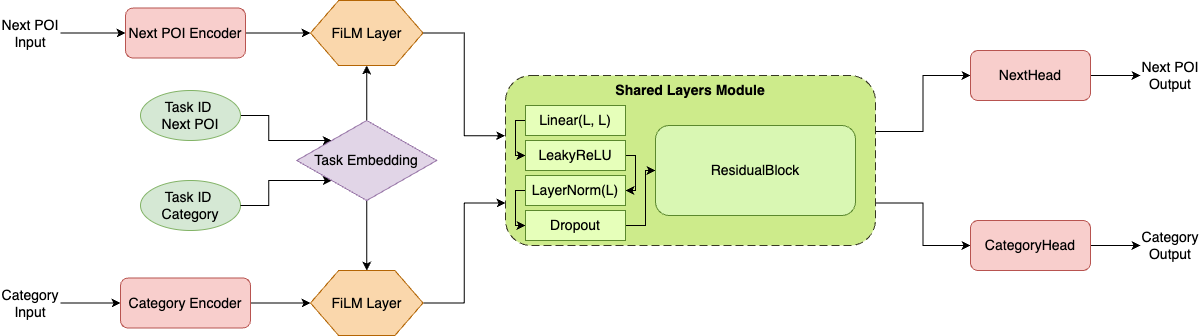
\includegraphics[width=\textwidth]{imgs/mtlnet_poi.drawio.png}
    \caption{The proposed Multi-Task Learning (MTL) architecture. Task-specific encoders process inputs for POI Category Classification and Next-POI Prediction. Feature-wise Linear Modulation (FiLM) layers adapt these features using learnable task embeddings. The modulated representations are then processed by a shared path of residual blocks. Finally, dedicated task-specific heads generate the respective outputs.}
    \label{fig:arch}
\end{figure*}
%
% Nash–MTL Optimizer
%
\subsection{Nash–MTL Optimizer}\label{sec:nash_mtl}

MTL necessitates a unified update direction that benefits all tasks, even when their gradients conflict. Nash-MTL formulates this as a cooperative $K$-player bargaining game\cite{nash}, where each task acts as an "agent" seeking to maximize its utility (loss reduction). The optimizer selects a step that is (i) beneficial to all tasks, (ii) scale-invariant to arbitrary loss re-weightings, and (iii) proportionally fair, ensuring no alternative direction increases one task's utility without decreasing the product of all utilities\cite{nash}. The unique solution satisfying these axioms is the Nash Bargaining Solution (NBS). This approach allows Nash-MTL to "negotiate" at each iteration, yielding a compromise descent direction that improves every loss while maximizing the joint progress of the entire system.

\paragraph*{Formal Formulation.}
Given task-specific objectives $\{\mathcal{L}_k(\boldsymbol{\theta})\}_{k=1}^{K}$ and their gradients $\mathbf{g}_k=\nabla_{\!\boldsymbol{\theta}}\mathcal{L}_k$ at current parameters $\boldsymbol{\theta}$, Nash-MTL frames gradient aggregation as a bargaining game to determine the common update direction \cite{nash}. The utility for each task $k$ is its signed improvement, $u_k(\Delta\boldsymbol{\theta})=\mathbf{g}_k^{\!\top}\!\Delta\boldsymbol{\theta}$, where $\Delta\boldsymbol{\theta}$ is the parameter update within an $\varepsilon$-ball \cite{nash}. The NBS is found by maximizing the weighted geometric mean of utilities:
\begin{equation}
\Delta\boldsymbol{\theta}^{*}\;=\;\argmax_{\Delta\boldsymbol{\theta}\in\mathcal{B}_\varepsilon}
\sum_{k=1}^{K}\!\log\!\bigl(u_k(\Delta\boldsymbol{\theta})\bigr)
\quad\text{s.t. }u_k(\Delta\boldsymbol{\theta})>0,\;\forall k.
\label{eq:nbs_objective}
\end{equation}
By setting $\Delta\boldsymbol{\theta}=\sum_{k}\alpha_k\mathbf{g}_k$ with positive weights $\boldsymbol{\alpha}$, the solution simplifies to solving the nonlinear system $\bigl(\mathbf{G}^{\!\top}\mathbf{G}\bigr)\boldsymbol{\alpha} \;=\; \boldsymbol{\alpha}^{-1}$ \cite{nash}, where $\mathbf{G}=\bigl[\mathbf{g}_1\,\ldots\,\mathbf{g}_K\bigr]$ \cite{nash}. The parameter update is then $\boldsymbol{\theta}^{(t+1)} =\boldsymbol{\theta}^{(t)}-\eta\,\mathbf{G}\boldsymbol{\alpha}$, with $\eta$ chosen to ensure monotonic loss decrease and convergence to a Pareto-stationary point \cite{nash}.

\paragraph*{Practical Aspects.}
Nash-MTL is architecture-agnostic and requires only two matrix-vector products per iteration. Its reliance on gradient signs rather than scales inherently balances heterogeneous tasks without manual re-weighting. For efficiency, task weights can be updated less frequently, significantly reducing runtime while maintaining performance~\cite{nash}.


\paragraph*{Parameter Partition.}
In our model (Figure~\ref{fig:arch}), we explicitly expose two disjoint parameter sets:
\[
\resizebox{\linewidth}{!}{$%
  \begin{aligned}
    \Theta_{\text{shared}}   &= \{\texttt{task\_emb},\texttt{film},\texttt{shared\_layers}\},\\
    \Theta_{\text{specific}} &= \{\texttt{category\_encoder},\texttt{next\_encoder},
                                 \texttt{CategoryHead},\texttt{NextHead}\}.
  \end{aligned}
$}
\]
This partition enables independent learning-rate scheduling or regularization if domain shifts between tasks emerge during fine-tuning.

The Nash-MTL optimizer was employed for its ability to aggregate tasks gradients in a balanced and principled manner, formulating the optimization process as a bargaining problem and aiming for joint progress across all tasks. In our evaluation, Nash-MTL was compared with different strategies, including PCGrad~\cite{yu2020pcgrad}  and an approach with no optimizer. Among these, it was found that Nash-MTL consistently yielded a better overall performance of the MTL model, with a lower combined multi-task loss, which supported our decision to adopt it as our choice of optimizer.


%
% Experimental Setup and Results
%
% Topicos a serem discutidos:
% 1 - Apresentar os dados do gowalla e as metricas de avaliação(De forma breve) //Felipe ✅
% 2 - Descutir sobre  os resultados do modelos MTL comparando com as baseslines 
%  - Discutir sobre o HMRMR como baseline do Category copiar do (Combining Recurrent and Graph Neural Networks to Predict the Next Place’s Category)
%  - Discutir sobre o MHA+PE(next) como baseline para o Next copiar do (Combining Recurrent and Graph Neural Networks to Predict the Next Place’s Category) ✅
% 3 - MTL converge mais rapido

% Section 3: Experimental Setup and Results
\section{Experimental Setup and Results}
\label{sec:experiments}

\subsection{Dataset and Evaluation Metrics}
\label{sec:method:single_task_heads}

To evaluate our model, we use a subset of the public \emph{Gowalla} check-in dataset, originally collected by Cho \textit{et al.}\,\cite{Cho2011}. We focus our analysis on the data from the U.S. state of Florida, which is one of the most active regions in the original dataset. This subset comprises a total of {$N_\text{users}$} users, {$N_\text{poi}$} unique Points-of-Interest (POIs), and {$N_\text{checkins}$} check-ins.

Following previous work, each POI is mapped to one of seven high-level categories: \emph{Community}, \emph{Entertainment}, \emph{Food}, \emph{Nightlife}, \emph{Outdoors}, \emph{Shopping}, and \emph{Travel}. These categories will be used for the POI category prediction task.

\paragraph*{Evaluation protocol}
To ensure a robust evaluation of our models, all experiments were conducted using a 5-fold cross-validation methodology. For every category, we report precision, recall, and $F_{1}$-score, and utilize the macro-average of these metrics to summarize overall performance. Class-wise metrics are crucial because category frequencies are highly skewed in real LBSN data.


\subsection{Discussion and Comparison with Established Models}
In this section, we discuss the performance of our proposed MTL model and its single-task (Single) counterpart. For a comprehensive evaluation, we selected two state-of-the-art approaches as baselines. The Human Mobility Representation Model (HMRM), introduced by Chen et al. (2020) \cite{chen2020modeling}, is designed for POI category classification. HMRM calculates POI embeddings by considering users' temporal visiting patterns and the co-occurrence of locations within an individual's historical trajectory. To quantify the relationship between locations and visiting times, it employs Point-wise Mutual Information (PMI). The model then utilizes matrix factorization techniques to generate latent representations (embeddings) from various inputs, and these embeddings are subsequently used to train a Support Vector Machine (SVM) for predicting POI categories. 

For the task of next POI category prediction, we compare our models against MHA+PE, a solution proposed by Zeng et al. (2019) \cite{zeng2019next}. This model enhances a recurrent neural network with a Multi-Head Attention (MHA) mechanism, originally developed for machine translation by Vaswani et al. (2017) \cite{vaswani2017attention}, and incorporates Positional Encoding (PE). The MHA mechanism allows the model to extract correlations from different parts of a sequence, effectively capturing the relevance of various elements within a user's trajectory, while positional encoding helps to propagate the order of records in a sequence.

\subsubsection{POI Category Classification}
As shown in Table \ref{table:cat}, both our MTL and Single models significantly outperform HMRM \cite{chen2020modeling} across all POI categories in terms of F1-score, precision, and recall. For instance, in the `Shopping' category, our MTL model achieves an F1-score of $62.51 \pm 0.94$ compared to HMRM's $46.69 \pm 0.81$. Similarly, for `Food', the MTL model scores $57.43 \pm 1.46$ against HMRM's $28.44 \pm 0.42$. While both MTL and Single models are competitive, the Single model shows marginally better F1-scores in several categories like `Community' ($53.11 \pm 0.58$) and `Outdoors' ($47.75 \pm 0.89$), whereas the MTL model excels in `Food' and `Shopping'. Overall, our approaches demonstrate a substantial improvement over the HMRM baseline for this task.

\begin{table}[htbp]
\caption{Table comparing the results of POI Classification for Florida}
\resizebox{\columnwidth}{!}{%
\begin{tabular}{|ll|r|r|r|}
\hline
\multicolumn{2}{|l|}{\textbf{}}                                  & \multicolumn{1}{c|}{\textbf{MTL}} & \multicolumn{1}{c|}{\textbf{Single}} & \multicolumn{1}{c|}{\textbf{HMRM}} \\ \hline
\multicolumn{1}{|l|}{\multirow{7}{*}{F1}}        & Community     & 52.13 ± 0.90                      & \textbf{53.11 ± 0.58}                & 20.25±0.52                         \\ \cline{2-5} 
\multicolumn{1}{|l|}{}                           & Entertainment & 41.44 ± 1.29                      & \textbf{41.73 ± 1.65}                & 13.07±1.14                         \\ \cline{2-5} 
\multicolumn{1}{|l|}{}                           & Food          & \textbf{57.43 ± 1.46}             & 56.70 ± 0.84                         & 28.44±0.42                         \\ \cline{2-5} 
\multicolumn{1}{|l|}{}                           & Nightlife     & 29.94 ± 2.27                      & \textbf{34.22 ± 2.08}                & 25.54±1.73                         \\ \cline{2-5} 
\multicolumn{1}{|l|}{}                           & Outdoors      & 47.19 ± 1.01                      & \textbf{47.75 ± 0.89}                & 16.11±0.68                         \\ \cline{2-5} 
\multicolumn{1}{|l|}{}                           & Shopping      & \textbf{62.51 ± 0.94}             & 61.88 ± 1.01                         & 46.69±0.81                         \\ \cline{2-5} 
\multicolumn{1}{|l|}{}                           & Travel        & 43.16 ± 1.43                      & \textbf{43.20 ± 1.94}                & 15.25±1.19                         \\ \hline
\multicolumn{1}{|l|}{\multirow{7}{*}{Precision}} & Community     & \textbf{51.39 ± 1.77}             & 49.54 ± 1.70                         & 21.13 ± 0.75                       \\ \cline{2-5} 
\multicolumn{1}{|l|}{}                           & Entertainment & 44.08 ± 1.46                      & \textbf{44.47 ± 3.66}                & 14.52 ± 1.34                       \\ \cline{2-5} 
\multicolumn{1}{|l|}{}                           & Food          & 58.05 ± 1.23                      & \textbf{59.04 ± 1.12}                & 48.94 ± 0.88                       \\ \cline{2-5} 
\multicolumn{1}{|l|}{}                           & Nightlife     & \textbf{36.07 ± 2.05}             & 32.52 ± 1.83                         & 18.34 ± 1.34                       \\ \cline{2-5} 
\multicolumn{1}{|l|}{}                           & Outdoors      & 46.39 ± 1.12                      & \textbf{47.74 ± 1.09}                & 13.00 ± 0.48                       \\ \cline{2-5} 
\multicolumn{1}{|l|}{}                           & Shopping      & 60.24 ± 1.21                      & \textbf{61.59 ± 1.44}                & 39.63 ± 0.82                       \\ \cline{2-5} 
\multicolumn{1}{|l|}{}                           & Travel        & \textbf{46.48 ± 1.12}             & 44.69 ± 4.89                         & 24.58 ± 1.91                       \\ \hline
\multicolumn{1}{|l|}{\multirow{7}{*}{Recall}}    & Community     & 52.93 ± 1.35                      & \textbf{57.37 ± 2.46}                & 19.48 ± 0.99                       \\ \cline{2-5} 
\multicolumn{1}{|l|}{}                           & Entertainment & 39.14 ± 1.69                      & \textbf{39.88 ± 4.93}                & 11.90 ± 1.08                       \\ \cline{2-5} 
\multicolumn{1}{|l|}{}                           & Food          & \textbf{56.99 ± 3.71}             & 54.60 ± 2.01                         & 20.05 ± 0.32                       \\ \cline{2-5} 
\multicolumn{1}{|l|}{}                           & Nightlife     & 25.80 ± 3.54                      & \textbf{36.77 ± 5.86}                & 42.13 ± 3.28                       \\ \cline{2-5} 
\multicolumn{1}{|l|}{}                           & Outdoors      & \textbf{48.09 ± 2.11}             & 47.79 ± 1.51                         & 21.27 ± 1.78                       \\ \cline{2-5} 
\multicolumn{1}{|l|}{}                           & Shopping      & \textbf{65.04 ± 2.69}             & 62.28 ± 2.83                         & 56.82 ± 0.98                       \\ \cline{2-5} 
\multicolumn{1}{|l|}{}                           & Travel        & 40.39 ± 2.73                      & \textbf{43.08 ± 7.15}                & 11.07 ± 0.95                       \\ \hline
\end{tabular}%
}
\label{table:cat}
\end{table}


\subsubsection{Next POI Category Prediction}
The results for next POI category prediction, detailed in Table \ref{table:next}, indicate a competitive performance landscape. The MHA+PE model \cite{zeng2019next} shows strong F1-scores in several categories, notably `Food' ($43.47 \pm 0.50$) and `Shopping' ($43.53 \pm 1.66$), outperforming our MTL and Single models in these instances. However, our MTL model achieves the best F1-score in `Travel' ($64.61 \pm 1.11$) and `Nightlife' ($22.07 \pm 0.52$), significantly surpassing MHA+PE in these categories. The Single model also shows competitive results, leading in `Entertainment' ($26.06 \pm 1.01$) and `Outdoors' ($22.45 \pm 0.81$). This suggests that while MHA+PE is highly effective for certain POI categories, our MTL and Single models offer superior or comparable performance in others, particularly where different sequential patterns might be leveraged. Also, it is important to notice that since we have an unbalanced result for the MTL and single, this could lead to the worse of other results.
\begin{table}[htbp]
\caption{Table comparing the results of Next POI Prediction for Florida}

\resizebox{\columnwidth}{!}{%
\begin{tabular}{|ll|r|r|r|}
\hline
\multicolumn{2}{|l|}{\textbf{}} & \multicolumn{1}{c|}{\textbf{MTL}} & \multicolumn{1}{c|}{\textbf{Single}} & \multicolumn{1}{c|}{\textbf{MHA+PE}} \\ \hline
\multicolumn{1}{|l|}{\multirow{7}{*}{F1}} & Community & 34.79 ± 1.05 & {\ul 34.90 ± 0.61} & \textbf{35.83±1.70} \\ \cline{2-5} 
\multicolumn{1}{|l|}{} & Entertainment & 24.21 ± 1.75 & \textbf{26.06 ± 1.01} & {\ul 25.48±0.86} \\ \cline{2-5} 
\multicolumn{1}{|l|}{} & Food & {\ul 28.06 ± 3.55} & 26.35 ± 2.97 & \textbf{43.47±0.50} \\ \cline{2-5} 
\multicolumn{1}{|l|}{} & Nightlife & \textbf{22.07 ± 0.52} & {\ul 21.79 ± 0.30} & 1.55±1.50 \\ \cline{2-5} 
\multicolumn{1}{|l|}{} & Outdoors & {\ul 21.61 ± 0.50} & \textbf{22.45 ± 0.81} & 12.56±1.94 \\ \cline{2-5} 
\multicolumn{1}{|l|}{} & Shopping & {\ul 42.58 ± 2.06} & 42.18 ± 1.13 & \textbf{43.53±1.66} \\ \cline{2-5} 
\multicolumn{1}{|l|}{} & Travel & \textbf{64.61 ± 1.11} & {\ul 64.32 ± 0.88} & 26.91±0.97 \\ \hline
\multicolumn{1}{|l|}{\multirow{7}{*}{Precision}} & Community & {\ul 30.22 ± 1.36} & 30.04 ± 1.08 & \textbf{42.59±1.48} \\ \cline{2-5} 
\multicolumn{1}{|l|}{} & Entertainment & {\ul 32.64 ± 2.55} & 28.63 ± 2.85 & \textbf{38.72±1.56} \\ \cline{2-5} 
\multicolumn{1}{|l|}{} & Food & 39.05 ± 0.70 & \textbf{39.87 ± 1.48} & 35.91±0.81 \\ \cline{2-5} 
\multicolumn{1}{|l|}{} & Nightlife & {\ul 17.71 ± 2.40} & 15.27 ± 0.67 & \textbf{39.67±23.94} \\ \cline{2-5} 
\multicolumn{1}{|l|}{} & Outdoors & {\ul 19.63 ± 2.93} & 19.50 ± 2.08 & \textbf{46.83±1.82} \\ \cline{2-5} 
\multicolumn{1}{|l|}{} & Shopping & {\ul 42.57 ± 0.78} & \textbf{43.47 ± 1.08} & 39.04±1.06 \\ \cline{2-5} 
\multicolumn{1}{|l|}{} & Travel & {\ul 60.64 ± 1.87} & \textbf{63.21 ± 0.67} & 36.64±1.74 \\ \hline
\multicolumn{1}{|l|}{\multirow{7}{*}{Recall}} & Community & 41.54 ± 5.27 & \textbf{41.92 ± 3.49} & 31.16±3.20 \\ \cline{2-5} 
\multicolumn{1}{|l|}{} & Entertainment & 19.52 ± 3.18 & \textbf{24.16 ± 2.16} & 19.05±1.25 \\ \cline{2-5} 
\multicolumn{1}{|l|}{} & Food & {\ul 22.19 ± 4.32} & 19.94 ± 3.75 & \textbf{55.12±1.46} \\ \cline{2-5} 
\multicolumn{1}{|l|}{} & Nightlife & 32.13 ± 9.47 & \textbf{38.35 ± 3.11} & 0.80±0.79 \\ \cline{2-5} 
\multicolumn{1}{|l|}{} & Outdoors & 25.06 ± 4.26 & \textbf{27.07 ± 3.40} & 7.30±1.32 \\ \cline{2-5} 
\multicolumn{1}{|l|}{} & Shopping & 42.87 ± 4.56 & 41.05 ± 2.33 & \textbf{49.37±3.74} \\ \cline{2-5} 
\multicolumn{1}{|l|}{} & Travel & \textbf{69.36 ± 4.15} & {\ul 65.52 ± 2.25} & 21.30±1.03 \\ \hline
\end{tabular}%
}

\label{table:next}
\end{table}

Overall, while our proposed models show strong performance in POI category classification against HMRM \cite{chen2020modeling}, the next POI category prediction task presents a more competitive landscape when compared against a sophisticated sequential model like MHA+PE \cite{zeng2019next}. Comparing the MTL and Single models directly reveals that the multi-task learning approach did not yield the anticipated substantial improvements over the single-task baseline across both tasks. Crucially, many of these observed differences in F1-scores are minor and often fall within the reported standard deviations, suggesting that, statistically, the performance of the MTL and Single models is largely comparable, without a clear, consistent, and significant advantage for the multi-task learning setup in these experiments.

\subsection{Convergence Comparison}
To further evaluate the practical implications of the MTL approach compared to single-task models, we conducted a convergence experiment. We measured the wall time, number of epochs, and Mega Floating Point Operations (MFLOPs) required for the MTL model and the individual single-task models (SingleClass and SinglePred) to reach predefined target average F1-scores. The target F1-score for the \textit{Category} prediction task was set to 47, and for the \textit{Next} POI category classification task, it was set to 32.2. These specific F1 values were chosen because they are close to the best-achieved results for each respective task, thereby representing a comparable and significant level of predictive performance for the models to attain. To ensure robust measurements for this experiment, all models were evaluated through a 5-fold cross-validation process. The specific metrics are detailed in Table \ref{table:convergence_comparison}.

\begin{table}[htbp]
\centering
\caption{Convergence metrics to reach target F1-score}
\begin{tabular}{|l|r|r|r|}
\hline
\textbf{Model}    & \textbf{Time(s)} & \textbf{Epochs} & \textbf{MFLOPs} \\ \hline
\textbf{Category} & 16.26            & 3.8             & 2.315           \\ \hline
\textbf{Next}     & 18.71            & 3.2             & 0.012           \\ \hline
\textbf{MTL}      & 80.88            & 3.2             & 0.234           \\ \hline
\end{tabular}
\label{table:convergence_comparison}
\end{table}



The results from this experiment were contrary to the potential expectation that an MTL framework might offer training efficiencies. Our findings indicated that the MTL model took substantially longer to converge to the target F1-scores. Specifically, the MTL approach required almost four times more wall time compared to the cumulative time of the individual single-task models. Furthermore, the computational cost, when considering MFLOPs, was roughly double for the MTL setup. This suggests that while attempting to learn multiple tasks simultaneously, the MTL model, in this configuration, incurred a significantly higher overhead in both time and computational resources. Given these observations, for deployment scenarios where convergence speed and computational efficiency are critical factors, employing separate, optimized single-task models would likely be a more convenient and resource-efficient strategy.\footnote{Experiments conducted on Apple M2 Pro (10-core CPU, 16-core GPU) with 32GB unified memory running macOS 15.5. Key software versions: Python 3.9.6, PyTorch 2.6.0.dev20241014+cpu, NumPy 1.26.4, scikit-learn 1.5.2, CVXPY 1.5.2. Training utilized PyTorch MPS backend for Apple Silicon acceleration.}


%

%
% Conclusion and Future Work
%
% Section 4: Conclusion and Future Work
\section{Conclusion and Future Work}
\label{sec:conclusion}

In this paper, we introduced a Multi-Task Learning (MTL) framework employing hard parameter-sharing, task-specific encoders, and FiLM layers to jointly address POI Category Classification and Next-POI Prediction using DGI-based POI embeddings.
%Our investigations revealed that while the proposed models, both single-task and MTL, significantly outperformed the HMRM baseline for POI Category Classification, the Next-POI Prediction task was more competitive against the MHA+PE state-of-the-art.

Essentially, the MTL approach did not consistently demonstrate superior performance over its single-task counterparts and exhibited higher computational demands in terms of convergence time and MFLOPs. These findings underscore that the anticipated benefits of MTL are not universally guaranteed and are highly dependent on task compatibility and architectural design.

The lack of significant improvement from the MTL model prompts an analysis of the potential underlying causes, especially since optimizers like Nash-MTL mitigated overt gradient conflicts. We hypothesize three primary factors contributed to this outcome:
\begin{itemize}
    \item \textbf{Subtle Negative Transfer due to Task Dissimilarity:} Although related, the two tasks possess fundamentally different natures. POI Category Classification is a static task that relies on the intrinsic, context-rich features of a single POI embedding. In contrast, Next-POI Prediction is a dynamic, sequential task that depends on capturing temporal patterns and transitions within a user's trajectory. The shared encoder may have been forced to learn a "compromise" representation that was not specialized enough for either task, thus failing to outperform the focused single-task models.
    \item \textbf{Task Difficulty and Representation Mismatch:} The performance gap between the two tasks (with category classification achieving higher F1-scores) suggests an imbalance in difficulty. The representation learned by the shared layers might have become biased towards the features required for the simpler, static classification task, inadvertently hindering its effectiveness for the more complex sequential prediction task. The shared representation may not have been rich enough to simultaneously encode both semantic properties and sequential dynamics effectively.
    \item \textbf{Architectural Restrictiveness:} Our choice of a hard parameter-sharing architecture, while efficient and strongly regularizing, may have been too restrictive for the tasks. The distinct nature of the tasks might require more flexible computational pathways. A single shared block may be insufficient to learn a representation that benefits both, suggesting that soft-sharing or expert-based models could be more appropriate.
\end{itemize}

These insights contribute to the broader understanding of MTL's practical challenges. Future research will proceed along several directions motivated by these hypotheses. We plan to explore alternative parameter-sharing mechanisms, such as \textbf{soft sharing (e.g., Cross-Stitch Networks) or Mixture-of-Experts (MoE) models}, to test the hypothesis that the hard-sharing architecture was overly restrictive. Furthermore, investigating \textbf{advanced multi-task optimizers and loss-balancing schemes} beyond gradient conflict mitigation could address the task difficulty imbalance. Finally, a deeper analysis of \textbf{task relatedness}, perhaps using techniques to measure feature representation overlap, could help quantify the degree of negative transfer and guide future architectural choices.

\section*{Acknowledgment} 
The authors would like to acknowledge the support of the Brazilian Ministry of Science, Technology and Innovations (MCTI), the Manna Team, Fundação Araucária, Softex, CNPq (Grant Number 421548/2022-3), and the Research Support Foundation of the State of Minas Gerais (FAPEMIG), and CAPES.

%
% REFERENCES
%
\bibliographystyle{IEEEtran}
\bibliography{references}



\end{document}
